\cxset{
 author block=false,
 name={},
 numbering=arabic,
 number font-size=\HUGE,
 number font-family=\sffamily,
 number font-weight=\bfseries,
 number before={},
 number dot=,
 number position=leftname,
 chapter font-family=\sffamily,
 chapter font-weight=\normalfont,
 chapter font-size=\small,
 number after={},
 chapter before={\vspace*{50pt}},
 chapter after={\par\vskip12pt},
 chapter color= black!90,
 number color=black!90,
 title beforeskip={},
 title afterskip={\vspace{30pt}},
 title before=,
 title after={\par},
 title font-family=\sffamily,
 title font-color= black!80,
 title font-weight=\bfseries,
 title font-size=\huge,
 section numbering = arabic,
 section numbering prefix = \thechapter.,}
\chapter{Introduction to style twenty seven }
\lipsum[3]

\medskip
\begin{figure}[ht]
\centering
\fbox{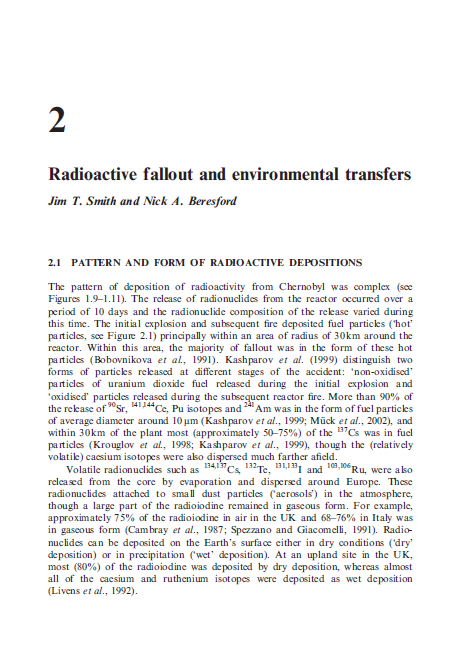
\includegraphics[width=0.5\textwidth]{./chapters/chapter27}}
\end{figure}

\section{PATHWAY AND FORM OF RADIOACTIVE DEPOSITIONS}
\@afterindentfalse

\lipsum[2-3]

